\documentclass [12pt]{article}
\usepackage{epsfig}
\usepackage{enumitem}
\usepackage{amsmath}
% \usepackage[color, leftbars]{changebar}
% \usepackage{fontawesome} 
% \usepackage{caption}
% \usepackage{subcaption}


\setlength{\textwidth}{6.5in}
\setlength{\textheight}{9in}
\setlength{\oddsidemargin}{0in}
\setlength{\evensidemargin}{0in}
\setlength{\topmargin}{-0.5in}

\setlength{\parindent}{0pt}

% \newtheorem{theorem}{Theorem}[section]
% \newtheorem{definition}[theorem]{Definition}
% \newtheorem{claim}[theorem]{Claim}
% \newtheorem{lemma}[theorem]{Lemma}
% \newtheorem{proof}[theorem]{Proof}

\newlength{\toppush}
\setlength{\toppush}{2\headheight}
\addtolength{\toppush}{\headsep}

\usepackage{hyperref}
\hypersetup{
    colorlinks=true,
    linkcolor=blue, % was previously black
    filecolor=magenta,
    urlcolor=blue,
    pdftitle={Template}
}
\urlstyle{same}


\def\subjnum{EE 156}
\def\subjname{Adv. Comp. Arch.}

\def\doheading#1#2#3{\vfill\eject\vspace*{-\toppush}%
  \vbox{\hbox to\textwidth{{\bf} \subjnum: \subjname \hfil Amy Bui}%
    \hbox to\textwidth{{\bf} Tufts University, Spring 2023 \hfil#3\strut}%
    \hrule}}

\newcommand{\htitle}[1]{\vspace*{3.25ex plus 1ex minus .2ex}%
\begin{center}
{\large\bf #1}
\end{center}} 

%%%%%%%%%%%%%%%%%%%%%%%%%%%%%%%%%%%%%%%%%%%%%%%%%%%%%%%%%%%%%%%%%%%

\begin{document}
\doheading{2}{title}{Noise Notes and PR} 
% \htitle{Paper Info}
% \bigskip 
% \bigskip 
%%%%%%%%%% begin text after this line %%%%%%%%%%%%%%

    \section{Necessity of Noise Modeling} %%%
        \begin{itemize}
            \item A quantum system has to involve some incoherence processes (measurements, random perturbations, etc), which ultimately makes the system probabilistic. So a noisy quantum system produces a random distribution of quantum states $| \psi_{i} \rangle$ with probability $p_{i}$ due to imprecise controls and environmental noise \cite{ding}.
            
            \item Start by modeling noise as a probability distribution over pure quantum states, $\{ p_i, | \psi_i \rangle \}$ \cite{ding}.
            \item 
        \end{itemize}

    %%%%%%%%%%%%%%%%%%%%%%%%%%%%%%%%%%%%%%%%%%%%%%%%%%%%%%%

    \section{Basic Noise Modeling}
        \begin{itemize}
            \item Unitary coupling transformation $U$ represents the impact on noise/the environment on a quantum state. $U$ is applied to both environment and syste, $\rho_{\text{env}} \otimes \rho_{\text{in}}$
            
                \begin{figure}[htb!]
                    \centering
                    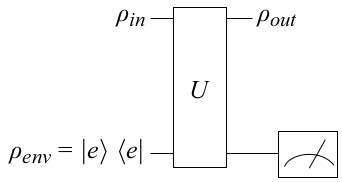
\includegraphics[width=0.25\textwidth]{images/unitaryCouplingTransformation.png}
                \end{figure}

            \item linear map: $\rho \rightarrow \mathcal{E}(\rho)$
            \item The unitary operator: $ \mathcal{E}(\rho) = U \rho U^{\dag} $
            \item operator form for entire unitary coupling evolution, with environment, $U$, and measurement. $U$ acts on both system and environment.  
                $$ \rho_{\text{in}} \rightarrow \rho_{\text{out}} = \textbf{tr}_{\text{env}}(U (\rho_{\text{env}} \otimes \rho_{\text{in}}) U^{\dag}) $$

            
            \item 
        \end{itemize}



    \section{Reference Formulas} %%%
        \begin{itemize}
            \item Quantum Circuit Model: For an $n$-qubit quantum system,
            $$ | \psi \rangle = \sum_{b\in\{0,1\}^n} \alpha_b | b \rangle $$
            Coefficient $\alpha_b$ is the amplitude of basis bit-string $b$. 

            \item The joint state of two separate quantum systems is represented with \emph{tensor product}, $| \psi_0 \rangle \otimes | \psi_1 \rangle$
            
            \item trace of a matrix is the sum of its diagonal elements, i.e. diagonal sum. $|e_i\rangle$  is the basis vector with 1 at the $i^{\text(th)}$ index, and 0 everywhere else: $$ \textbf{tr}(A) = \sum_i A_{ii} = \sum_i | e_i \rangle A | e_i \rangle  $$
            
            \item density matrix representation, $\rho$, is how mixed state is represented: $$ \rho = \sum_i p_i | \psi_i \rangle | \psi_i \rangle $$
            
            \item trace and density matrix helps define the fidelity metric for quantifying the quality of a quantum state: $ \textbf{tr}(\rho \sigma)  $, where $\sigma$ is actual quantum state, versus the density matrix or ``correct'' quantum state \cite{resch21}.
        \end{itemize}
    %%%%%%%%%%%%%%%%%%%%%%%%%%%%%%%%%%%%%%%%%%%%%%%%%%%%%%%


    \section{Paper Overviews} %%%

    \begin{itemize}
        \item Salonik Resch and Ulya R. Karpuzcu. 2021. \href{https://dl-acm-org.ezproxy.library.tufts.edu/doi/10.1145/3464420}{Benchmarking Quantum Computers and the Impact of Quantum Noise}. ACM Comput. Surv. 54, 7, Article 142 (September 2022), 35 pages.
            \begin{itemize}
                \item Details benchmarking quantum computers from a computer architecture perspective and the challenges, as well as the significance and complexity of things that have to be considered when benchmarking, such as noise model (and ability to simulate and/or characterize), target application, and performance metrics. The authors categorize some physical noise sources (environment or other qubits), and overviews some noise models (Stochastic Pauli Noise, Coherent Noise, Amplitude/Phase Damping) and references other related works that cover these models. They also go over different metrics and how different ones may be preferred (process fidelity, average gate fidelity/infidelity, trace distance, Hellinger fidelity). They run benchmarks on a few quantum benchmarks and use the process fidelity metric to illustrate the impact of noise.
            \end{itemize}

        \item 
    \end{itemize}

    %%%%%%%%%%%%%%%%%%%%%%%%%%%%%%%%%%%%%%%%%%%%%%%%%%%%%%%%%%%%%%%%





\begin{thebibliography}{1}
    \bibitem[ding2020]{ding}Y. Ding, F. Chong. \href{https://link.springer.com/book/10.1007/978-3-031-01765-0}{Quantum Computer Systems: Research for Noisy Intermediate-Scale Quantum Computers}. Springer Cham. Synthesis Lectures on Computer Architecture. 2020

    \bibitem[resch21]{resch21}Salonik Resch and Ulya R. Karpuzcu. 2021. \href{https://dl-acm-org.ezproxy.library.tufts.edu/doi/10.1145/3464420}{Benchmarking Quantum Computers and the Impact of Quantum Noise}. ACM Comput. Surv. 54, 7, Article 142 (September 2022), 35 pages.

    \bibitem[barnes17]{barnes17}Barnes, Jeff P. and Trout, Colin J. and Lucarelli, Dennis and Clader, B. D.\href{https://arxiv.org/abs/1704.03961}{Quantum error-correction failure distributions: Comparison of coherent and stochastic error models}. American Physical Society. Phys. Rev. A, Vol.. 95, Issue 6 (June 2017).

    \bibitem[beale18]{beale18}Stefanie J. Beale, Joel J. Wallman, Mauricio Gutiérrez, Kenneth R. Brown, and Raymond Laflamme. 2018. \href{https://link.aps.org/accepted/10.1103/PhysRevLett.121.190501}{Quantum
    error correction decoheres noise}. Phys. Rev. Lett. 121, 19 (2018), 190501.

    \bibitem[bravyi18]{bravyi18}Sergey Bravyi, Matthias Englbrecht, Robert König, and Nolan Peard. 2018. \href{https://www.nature.com/articles/s41534-018-0106-y}{Correcting coherent errors with surface
    codes}. npj Quant. Inf. 4, 1 (2018), 55.

    \bibitem[duckering2020]{duckering2020}C. Duckering, J. M. Baker, D. I. Schuster and F. T. Chong, "\href{https://ieeexplore-ieee-org.ezproxy.library.tufts.edu/document/9251988}{Virtualized Logical Qubits: A 2.5D Architecture for Error-Corrected Quantum Computing}," 2020 53rd Annual IEEE/ACM International Symposium on Microarchitecture (MICRO), Athens, Greece, 2020, pp. 173-185, doi: 10.1109/MICRO50266.2020.00026.

    \bibitem[wallman15]{wallman15}Joel Wallman, Chris Granade, Robin Harper, and Steven T. Flammia. 2015. Estimating the coherence of noise. New J. Phys. 17, 11 (2015), 113020.

    \bibitem[nickerson19]{nickerson19}Naomi H. Nickerson and Benjamin J. Brown. 2019. \href{https://arxiv.org/abs/1712.00502}{Analysing correlated noise on the surface code using adaptive decoding algorithms}. Quantum 3 (2019), 131.
\end{thebibliography}
%%%%%%%%%%%%%%%%%%%%%%%%%%%%%%%%%%%%%%%%%%%%%%%%%%%%%%%%%%%%%%%%%%%%%%
\end{document}
%%%%%%%%%%%%%%%%%%%%%%%%%%%%%%%%%%%%%%%%%%%%%%%%%%%%%%%%%%%%%%%%%%%%%%

